%=========================================================================
% (c) 2011, 2012 Josef Lusticky

\section{Network communication}
Thanks to uIP, described in section~\ref{sec:contiki-uip},
the network communication is not a matter for Contiki OS.
% 1 - see implementation/communication.tex
A problem might be a possible packet loss when communication uses UDP on transport layer.
The reason why this can happen often is explained in section~\ref{sec:contiki-uip}.
% 2
In NTP unicast mode, the packet loss might occur either for client's query to server
or for server's response to client.
If the client's query loss occurs, no server response will be sent.
Similarly, if the server's response loss occurs, no message will be received by the client.
Not to block a whole system till the response arrives
is therefore a desired behaviour of the client.

AVR Raven features IEEE~802.15.4 (Low-Rate Wireless Personal Area Networks) link layer support.
On top of this layer, an adaptation layer called 6LoWPAN (IPv6 over Low power Wireless Personal Area Networks)
is used to communicate over IPv6 by Contiki.
The 6LoWPAN layer is needed, because IPv6 requires support of much larger packet
sizes than the largest IEEE 802.15.4 frame size
(MTU on 802.15.4 links is 127 bytes,
whereas IPv6 mandates links with MTU of at least 1280 bytes)~\cite{interconnecting}.
In conjunction with RZ~USB Stick, the network connection with desktop PC can be established.
This USB Stick can be loaded with a firmware automatically translating
Ethernet packets to 802.15.4 packets and vice versa.
The firmware is distributed together with Contiki and
is to be found in {\it{/platform/avr-ravenusb/}} directory.
Figure~\ref{fig:design-6lowpan} show a complete hierarchy of network layers
concerned with NTP communication.
\begin{figure}
  \centering
  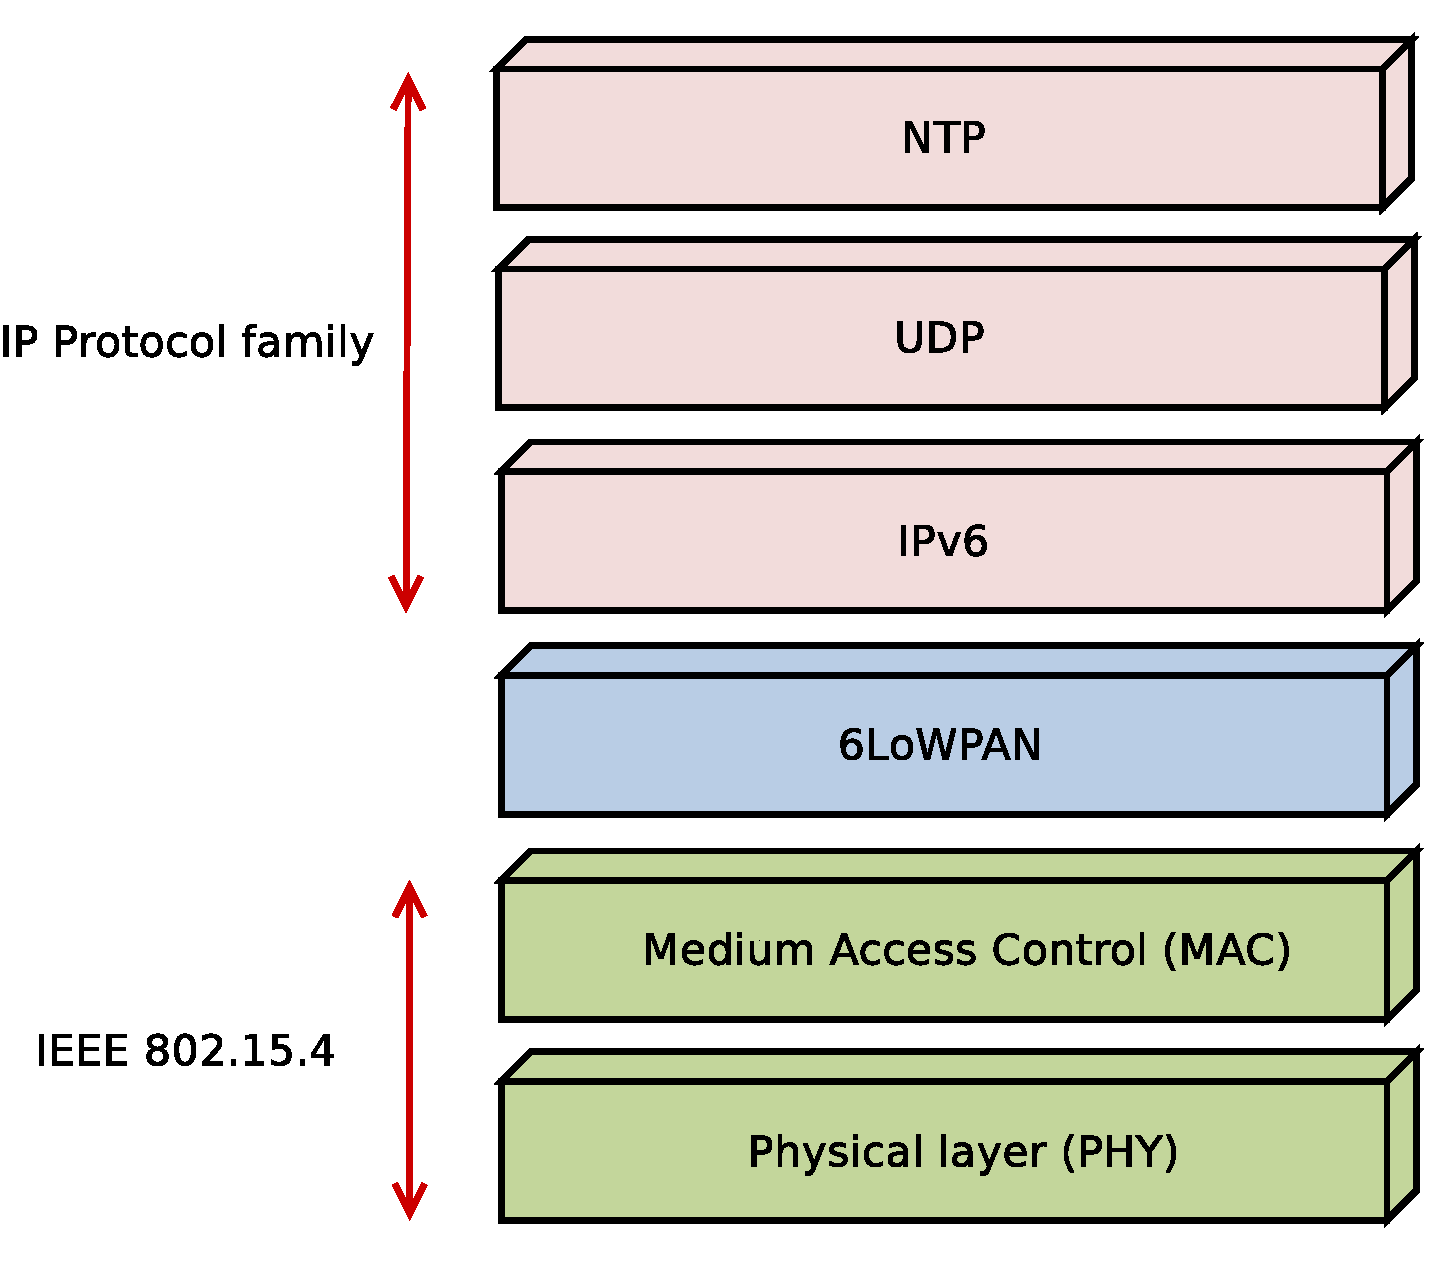
\includegraphics[width=9cm,keepaspectratio]{fig/6lowpan.pdf}
  \caption{Communication stack with 6lowpan layer}
  \label{fig:design-6lowpan}
  \bigskip
\end{figure}

Contiki supports broadcast packets as well as sending multicast packets~\cite{contiki-docs}.
An implementation of NTP broadcast mode is therefore also possible.
Joining multicast groups through Internet Group Management Protocol (IGMP)
and receiving non-local multicast packets
was not supported at the time of writing~\cite{contiki-docs}.
Contiki is also able to use Domain Name System for IPv4 address resolution.
DNS resolution of IPv6 addresses was not implemented in Contiki OS
at the time of writing~\cite{contiki-docs}.
